\documentclass[a4paper]{article}

\usepackage{inputenc}
\usepackage[british,UKenglish]{babel}
\usepackage{amsmath}
%\usepackage{titlesec}
\usepackage{color}
\usepackage{graphicx}
\usepackage{fancyref}
\usepackage{hyperref}
\usepackage{float}
\usepackage{scrextend}
\usepackage{setspace}
\usepackage{xargs}
\usepackage{multicol}
\usepackage{nameref}

\usepackage{sectsty}
\usepackage{multicol}
\usepackage{multirow}
\usepackage[procnames]{listings}
\usepackage{appendix}

\newcommand\tab[1][1cm]{\hspace*{#1}}
\hypersetup{colorlinks=true, linkcolor=black}
\interfootnotelinepenalty=10000

\newcommand{\cleancode}[1]{\begin{addmargin}[3em]{3em}\texttt{\textcolor{cleanOrange}{#1}}\end{addmargin}}
\newcommand{\cleanstyle}[1]{\text{\textcolor{cleanOrange}{\texttt{#1}}}}


\usepackage[colorinlistoftodos,prependcaption,textsize=footnotesize]{todonotes}
\newcommandx{\commred}[2][1=]{\textcolor{Red}
{\todo[linecolor=red,backgroundcolor=red!25,bordercolor=red,#1]{#2}}}
\newcommandx{\commblue}[2][1=]{\textcolor{Blue}
{\todo[linecolor=blue,backgroundcolor=blue!25,bordercolor=blue,#1]{#2}}}
\newcommandx{\commgreen}[2][1=]{\textcolor{OliveGreen}{\todo[linecolor=OliveGreen,backgroundcolor=OliveGreen!25,bordercolor=OliveGreen,#1]{#2}}}
\newcommandx{\commpurp}[2][1=]{\textcolor{Plum}{\todo[linecolor=Plum,backgroundcolor=Plum!25,bordercolor=Plum,#1]{#2}}}

\def\code#1{{\tt #1}}

\def\note#1{\noindent{\bf [Note: #1]}}

\makeatletter
%% The "\@seccntformat" command is an auxiliary command
%% (see pp. 26f. of 'The LaTeX Companion,' 2nd. ed.)
\def\@seccntformat#1{\@ifundefined{#1@cntformat}%
   {\csname the#1\endcsname\quad}  % default
   {\csname #1@cntformat\endcsname}% enable individual control
}
\let\oldappendix\appendix %% save current definition of \appendix
\renewcommand\appendix{%
    \oldappendix
    \newcommand{\section@cntformat}{\appendixname~\thesection\quad}
}
\makeatother


% "define" Scala
\usepackage[T1]{fontenc}  
\usepackage[scaled=0.82]{beramono}  
\usepackage{microtype} 

\sbox0{\small\ttfamily A}
\edef\mybasewidth{\the\wd0 }

\lstdefinelanguage{scala}{
  morekeywords={abstract,case,catch,class,def,%
    do,else,extends,false,final,finally,%
    for,if,implicit,import,match,mixin,%
    new,null,object,override,package,%
    private,protected,requires,return,sealed,%
    super,this,throw,trait,true,try,%
    type,val,var,while,with,yield},
  sensitive=true,
  morecomment=[l]{//},
  morecomment=[n]{/*}{*/},
  morestring=[b]",
  morestring=[b]',
  morestring=[b]"""
}

\usepackage{color}
\definecolor{dkgreen}{rgb}{0,0.6,0}
\definecolor{gray}{rgb}{0.5,0.5,0.5}
\definecolor{mauve}{rgb}{0.58,0,0.82}

% Default settings for code listings
\lstset{frame=tb,
  language=scala,
  aboveskip=3mm,
  belowskip=3mm,
  showstringspaces=false,
  columns=fixed, % basewidth=\mybasewidth,
  basicstyle={\small\ttfamily},
  numbers=none,
  numberstyle=\footnotesize\color{gray},
  % identifierstyle=\color{red},
  keywordstyle=\color{blue},
  commentstyle=\color{dkgreen},
  stringstyle=\color{mauve},
  frame=single,
  breaklines=true,
  breakatwhitespace=true,
  procnamekeys={def, val, var, class, trait, object, extends},
  procnamestyle=\ttfamily\color{red},
  tabsize=2
}

\lstnewenvironment{scala}[1][]
{\lstset{language=scala,#1}}
{}
\lstnewenvironment{cpp}[1][]
{\lstset{language=C++,#1}}
{}
\lstnewenvironment{bash}[1][]
{\lstset{language=bash,#1}}
{}
\lstnewenvironment{verilog}[1][]
{\lstset{language=verilog,#1}}
{}



%代码段设置
\lstset{numbers=left,
basicstyle=\tiny,
numberstyle=\tiny,
keywordstyle=\color{blue!70},
commentstyle=\color{red!50!green!50!blue!50},
frame=single, rulesepcolor=\color{red!20!green!20!blue!20},
escapeinside=``
}

\graphicspath{ {images/} }
\usepackage{ctex}
\usepackage{graphicx}
\usepackage{color,framed}%文本框
\usepackage{listings}
\usepackage{caption}
\usepackage{amssymb}
\usepackage{enumerate}
\usepackage{xcolor}
\usepackage{bm} 
\usepackage{lastpage}%获得总页数
\usepackage{fancyhdr}
\usepackage{tabularx}  
\usepackage{geometry}
\usepackage{graphics}
\usepackage{subfigure}
\usepackage{float}
\usepackage{pdfpages}
\usepackage{pgfplots}
\pgfplotsset{width=10cm,compat=1.9}
\usepackage{multirow}
\usepackage{footnote}
\usepackage{booktabs}

%-----------------------伪代码------------------
\usepackage{algorithm}  
\usepackage{algorithmicx}  
\usepackage{algpseudocode}  
\floatname{algorithm}{Algorithm}  
\renewcommand{\algorithmicrequire}{\textbf{Input:}}  
\renewcommand{\algorithmicensure}{\textbf{Output:}} 
\usepackage{lipsum}  
\makeatletter
\newenvironment{breakablealgorithm}
  {% \begin{breakablealgorithm}
  \begin{center}
     \refstepcounter{algorithm}% New algorithm
     \hrule height.8pt depth0pt \kern2pt% \@fs@pre for \@fs@ruled
     \renewcommand{\caption}[2][\relax]{% Make a new \caption
      {\raggedright\textbf{\ALG@name~\thealgorithm} ##2\par}%
      \ifx\relax##1\relax % #1 is \relax
         \addcontentsline{loa}{algorithm}{\protect\numberline{\thealgorithm}##2}%
      \else % #1 is not \relax
         \addcontentsline{loa}{algorithm}{\protect\numberline{\thealgorithm}##1}%
      \fi
      \kern2pt\hrule\kern2pt
     }
  }{% \end{breakablealgorithm}
     \kern2pt\hrule\relax% \@fs@post for \@fs@ruled
  \end{center}
  }
\makeatother
%------------------------代码-------------------
\usepackage{xcolor} 
\usepackage{listings} 
\lstset{ 
breaklines,%自动换行
basicstyle=\small\ttfamily,
escapeinside=``,
keywordstyle=\color{blue!70}\bfseries,
commentstyle=\color{red!50!green!50!blue!50},
stringstyle=\color{red}\ttfamily,
extendedchars=false,
linewidth=\textwidth,
numbers=left,
numberstyle=\tiny\color{blue!50},
frame=trbl,
rulesepcolor=\color{red!20!green!20!blue!20},
showstringspaces=false,
tabsize=4,
captionpos=b
}

% 定义更多语言的关键词高亮
\lstdefinelanguage{Python}{
    keywords={def,class,if,else,elif,for,while,try,except,import,from,as,return,break,continue,pass,with,yield,lambda,global,nonlocal,True,False,None},
    keywordstyle=\color{blue!70}\bfseries,
    sensitive=true,
    comment=[l]{\#},
    string=[s]{'}{'},
    morestring=[s]{"}{"}
}

%-------------------------页面边距--------------
\geometry{a4paper,left=2.3cm,right=2.3cm,top=2.7cm,bottom=2.7cm}
%-------------------------页眉页脚--------------
\usepackage{fancyhdr}
\pagestyle{fancy}
\lhead{\kaishu \leftmark}
% \chead{}
\rhead{\kaishu 并行程序设计实验报告}%加粗\bfseries  
\lfoot{}
\cfoot{\thepage}
\rfoot{}
\renewcommand{\headrulewidth}{0.1pt}  
\renewcommand{\footrulewidth}{0pt}%去掉横线
\newcommand{\HRule}{\rule{\linewidth}{0.5mm}}%标题横线
\newcommand{\HRulegrossa}{\rule{\linewidth}{1.2mm}}
\setlength{\textfloatsep}{10mm}%设置图片的前后间距
%--------------------文档内容--------------------

\usepackage{xurl}
\renewcommand{\UrlFont}{\ttfamily\color{blue}\small}

% 定义中英文摘要环境
\makeatletter
% 中文摘要环境
\newenvironment{cnabstract}{
    \par\small
    \noindent\mbox{}\par\vspace{-\baselineskip}
    \par\songti\parindent 2em
    }
    {\par\vspace{1em}}

% 英文摘要环境
\newenvironment{enabstract}{
    \par\small
    \noindent\mbox{}\par\vspace{-\baselineskip}
    \par\parindent 2em
    }
    {\par\vspace{1em}}
\makeatother

\begin{document}
\renewcommand{\contentsname}{目\ 录}
\renewcommand{\appendixname}{附录}
\renewcommand{\appendixpagename}{附录}
\renewcommand{\refname}{参考文献} 
\renewcommand{\figurename}{图}
\renewcommand{\tablename}{表}

%-------------------------封面----------------
\begin{titlepage}
    \begin{center}
    
\includegraphics[width=0.8\textwidth]{fig/NKU.png}\\[1cm]
    \vspace{20mm}
		\textbf{\huge\textbf{\kaishu{计算机学院}}}\\[0.5cm]
		\textbf{\huge{\kaishu{并行程序设计实验报告}}}\\[2.3cm]
		\textbf{\Huge\textbf{\kaishu{基于GPU的NTT多项式乘法并行优化}}}

		\vspace{\fill}
    
    % \textbf{\Large \textbf{并行程序设计期末实验报告}}\\[0.8cm]
    % \HRule \\[0.9cm]
    % \HRule \\[2.0cm]
    \centering
    \textsc{\LARGE \kaishu{姓名\ :\ 廖望}}\\[0.5cm]
    \textsc{\LARGE \kaishu{学号\ :\ 2210556}}\\[0.5cm]
    \textsc{\LARGE \kaishu{专业\ :\ 计算机科学与技术}}\\[0.5cm]
    
    \vfill
    {\Large 2025年6月28日}
    \end{center}
\end{titlepage}

% 中文摘要
\clearpage
\phantomsection
\begin{center}{\zihao{4}\songti\bfseries{摘\quad 要}}\end{center}\par\vspace{0.5em}
\addcontentsline{toc}{section}{摘要}
\begin{cnabstract}
本项目旨在利用NVIDIA GPU的大规模并行计算能力,对基于快速数论变换(NTT)的多项式乘法进行性能优化。实验在CUDA平台上实现并优化了NTT算法,通过预计算并一次性拷贝旋转因子、采用模板化内核设计等策略,显著降低了数据传输和计算开销。我们重点对比了朴素模乘、Barrett约减和Montgomery约减三种不同模乘算法在GPU上的性能表现。实验结果表明,与CPU串行实现相比,经过优化的GPU版本取得了高达78倍的性能加速,其中Montgomery约减方法表现最佳,充分展示了算法与硬件协同优化在解决计算密集型问题上的巨大潜力。代码仓库可访问:\href{https://github.com/aokimi0/parallel-programming}{GitHub}。

\vspace{1em}
\noindent\textbf{关键词:}并行计算; NTT; 性能优化; GPU; CUDA; Montgomery约减
\end{cnabstract}

% 英文摘要
\phantomsection
\begin{center}{\zihao{4}\bfseries{Abstract}}\end{center}\par\vspace{0.5em}
\addcontentsline{toc}{section}{Abstract}
\begin{enabstract}
This project aims to leverage the massively parallel computing power of NVIDIA GPUs to optimize the performance of polynomial multiplication based on the Number Theoretic Transform (NTT). The experiment implements and optimizes the NTT algorithm on the CUDA platform. By pre-computing and batch-copying twiddle factors and employing a templated kernel design, data transfer and computational overheads were significantly reduced. We focused on comparing the performance of three different modular multiplication algorithms on the GPU: naive, Barrett reduction, and Montgomery reduction. The results show that the optimized GPU version achieves a speedup of up to 78x compared to the serial CPU implementation, with the Montgomery reduction method performing the best. This demonstrates the immense potential of algorithm-hardware co-optimization in solving computationally intensive problems. Full code is available at: \href{https://github.com/aokimi0/parallel-programming}{GitHub}.

\vspace{1em}
\noindent\textbf{Keywords:} Parallel Computing; NTT; Performance Optimization; GPU; CUDA; Montgomery Reduction
\end{enabstract}

% 生成目录
\clearpage
\tableofcontents
\newpage

% 正文开始
\section{引言}
多项式乘法是数字信号处理、现代密码学等领域的关键计算任务。传统的 $O(n^2)$ 算法在处理大规模多项式时效率低下。为此,学术界和工业界普遍采用基于快速傅里叶变换(FFT)的 $O(n \log n)$ 算法。然而,FFT依赖于浮点运算,存在精度误差问题。

\textbf{快速数论变换(NTT)}通过在整数有限域上进行计算,完美地解决了FFT的精度问题,同时保持了 $O(n \log n)$ 的高效率,成为高精度、高性能多项式乘法,特别是在密码学应用中的理想选择。

本次实验的核心目标是利用NVIDIA GPU的大规模并行计算能力,对NTT算法进行加速。我们将实现一个CUDA版本的NTT,并通过优化数据传输、内存访问以及核心的模乘运算(对比朴素、Barrett、Montgomery三种方法),最终量化评估GPU并行版本相对于CPU串行版本的加速效果,并分析不同优化策略带来的性能增益。

\section{实验原理}
\subsection{快速数论变换 (NTT) 原理简述}
NTT是快速傅里叶变换(FFT)在有限域上的变体,它利用有限域中的"原根"替代复数单位根,将多项式乘法中的卷积运算转化为点值乘法,从而将时间复杂度从 \(O(n^2)\) 降低到 \(O(n \log n)\)。NTT的核心运算是蝶形运算,其迭代形式如下:对于长度为 \texttt{len} 的当前变换阶段和旋转因子 \texttt{w}:
\[ u = a[i] \]
\[ v = (a[i + len/2] \cdot w) \pmod{mod} \]
\[ a[i] = (u + v) \pmod{mod} \]
\[ a[i + len/2] = (u - v) \pmod{mod} \]
在NTT的每个阶段中,所有蝶形运算都是数据独立的,这为大规模并行化提供了理论基础。本次实验将使用一个纯C++串行实现的NTT算法作为性能基准,以衡量后续GPU优化的加速效果。

\subsection{CUDA 并行模型与实验环境}
CUDA采用\texttt{Grid-Block-Thread}的三级并行模型。一个CUDA内核(Kernel)以一个Grid的形式启动,Grid由多个Block组成,每个Block又由多个Thread组成。在本次实验中,我们将NTT的蝶形运算映射到CUDA线程上,以实现最大程度的并行。

实验环境如下:
\begin{itemize}
    \item \textbf{操作系统}: Ubuntu 24.04 (on WSL2)
    \item \textbf{处理器 (CPU)}: Intel Core i5-12500H
    \item \textbf{图形处理器 (GPU)}: NVIDIA GeForce RTX 3050 Ti Laptop GPU
    \item \textbf{编程语言}: C++, CUDA C++
    \item \textbf{编译器}: g++, nvcc 11.8
    \item \textbf{CUDA Toolkit}: 11.8
\end{itemize}

\subsection{关键优化原理:模乘约减}
在NTT中,模乘和模加/减是最高频的运算。由于\texttt{\%}取模运算符在硬件层面通常对应一个开销较大的\texttt{div}指令,优化模乘运算是提升NTT性能的关键。本次实验对比了三种方法:
\begin{enumerate}
    \item \textbf{朴素模乘 (Naive)}: 直接使用 \texttt{(a * b) \% mod}。这在代码上最简单,但性能最差。
    \item \textbf{Barrett约减 (Barrett Reduction)}: 通过预计算一个常数 \(\mu = \lfloor 2^k / m \rfloor\),将取模运算转换为两次乘法、一次移位和几次加减法。这避免了代价高昂的除法指令。其核心思想是 \texttt{a \% m = a - m * floor(a / m)},并用乘法和移位高效地计算 \texttt{floor(a/m)} 的近似值。
    \item \textbf{Montgomery约减 (Montgomery Reduction)}: 将所有操作数转换到一个特殊的"Montgomery域"中。在这个域内,模乘的计算效率非常高。其代价是在进入和离开Montgomery域时需要进行额外的转换。对于需要大量连续模乘的算法(如NTT),这个初始开销可以被摊销,从而获得显著的性能提升。
\end{enumerate}

\section{GPU 设计与实现}
\subsection{总体流程}
整个GPU加速的多项式乘法流程如下:
\begin{enumerate}
    \item \textbf{数据准备 (Host)}: 将两个输入多项式\texttt{poly1}和\texttt{poly2}补零,使其长度\texttt{n}扩展到大于等于$deg(\texttt{poly1}) + deg(\texttt{poly2}) - 1$的最小2的幂次。
    \item \textbf{位逆序 (Host)}: 对两个多项式的系数向量进行位逆序重排,以适应NTT迭代算法的输入要求。
    \item \textbf{内存拷贝 (H2D)}: 将重排后的系数向量从主机内存(Host)拷贝到设备内存(Device)。
    \item \textbf{正向NTT (Device)}: 在GPU上对两个系数向量分别执行正向NTT。
    \item \textbf{逐点相乘 (Device)}: 在GPU上将两个NTT变换后的结果向量进行逐点相乘。
    \item \textbf{逆向NTT (Device)}: 在GPU上对逐点相乘的结果执行逆向NTT。
    \item \textbf{最终缩放 (Device)}: 对逆向NTT的结果乘以 \(n^{-1} \pmod{mod}\),得到最终的多项式系数。
    \item \textbf{结果拷贝 (D2H)}: 将计算结果从设备内存拷贝回主机内存。
\end{enumerate}

\subsection{CUDA内核设计}
\subsubsection{模板化内核}
为了优雅地实现和对比三种不同的模乘算法,我们设计了模板化的CUDA内核。通过C++模板,我们可以编写一份通用的内核代码,模乘的具体实现由传入的\texttt{Reducer}结构体(如\texttt{BarrettReducer}, \texttt{MontgomeryReducer})决定。
\begin{lstlisting}[language=C++]
template<typename Reducer>
__global__ void ntt_kernel_optimized(ll* a, const ll* twiddles, int len, int n, const Reducer reducer) {
    int tidx = blockIdx.x * blockDim.x + threadIdx.x;
    // ... index calculation ...
    
    if (i < n) {
        ll w = twiddles[butterfly_idx_in_grp];
        ll u = a[i];
        // 使用Reducer进行模乘
        ll v = reducer.multiply(a[i + len / 2], w); 
        
        // ... butterfly operation ...
    }
}
\end{lstlisting}
这种设计不仅代码复用性高,而且编译器在编译时会为每种Reducer生成高度优化的特定代码,没有运行时开销。

\subsubsection{线程映射}
在NTT的每个阶段,有\texttt{n/2}个蝶形运算需要执行。我们启动\texttt{n/2}个线程(通过计算合适的\texttt{block}和\texttt{thread}数量),每个线程的全局ID \texttt{tidx} 被唯一地映射到一个蝶形运算上。
\begin{lstlisting}[language=C++]
// tidx范围是 [0, n/2 - 1]
int butterfly_grp_idx = tidx / (len / 2);      // 计算当前线程属于哪个蝶形运算组
int butterfly_idx_in_grp = tidx % (len / 2); // 计算当前线程在组内的索引
int i = butterfly_grp_idx * len + butterfly_idx_in_grp; // 计算蝶形运算的左侧操作数索引
\end{lstlisting}
这样保证了所有蝶形运算都能被并行处理,且没有线程冲突。

\subsection{旋转因子优化}
一个朴素的实现可能在NTT的每个阶段循环中都在主机端计算旋转因子,然后将其拷贝到设备端。这会导致多次小数据量的H2D拷贝,开销巨大。我们采用了显著的优化策略:
\begin{enumerate}
    \item \textbf{一次性预计算}: 在主机端,一次性计算出所有NTT阶段所需要的\textbf{全部}旋转因子。
    \item \textbf{一次性拷贝}: 将所有旋转因子存入一个连续的\texttt{vector}中,然后通过一次\texttt{cudaMemcpy}操作将其全部拷贝到GPU的全局内存中。
    \item \textbf{偏移量访问}: 在每个NTT阶段的内核中,通过指针偏移量访问当前阶段所需的旋转因子子集。
\end{enumerate}
这种方式将H2D通信开销从 \(O(\log n)\) 次降低到1次,极大地提升了整体性能。

\section{实验结果与分析}
\subsection{正确性验证}
我们通过将GPU版本的计算结果与经过验证的CPU串行版本的结果进行逐一比对,来确保GPU实现的正确性。在所有测试用例中,三种GPU方法(Naive, Barrett, Montgomery)的计算结果均与CPU版本完全一致,验证了实现的正确性。

\subsection{性能对比}
我们使用 \texttt{cudaEvent} 来精确测量GPU内核的执行时间,并使用\texttt{std::chrono}测量CPU串行代码的执行时间。实验在一个包含\texttt{n=131072}个系数的多项式上进行,四个基准版本的性能对比如下。

\begin{table}[H]
    \centering
    \caption{CPU与GPU不同优化策略性能对比 (n=131072)}
    \label{tab:gpu_perf_summary}
    \begin{tabular}{llc|l}
    \toprule
    \textbf{实现方式} & \textbf{核心技术} & \textbf{执行时间 (ms)} & \textbf{加速比 vs CPU Serial} \\
    \midrule
    CPU Serial     & 串行C++ & 1520.7        & 1.0x                 \\
    GPU Naive      & CUDA + 朴素模乘 & 45.3          & 33.6x                \\
    GPU Barrett    & CUDA + Barrett约减 & 28.9          & 52.6x                \\
    GPU Montgomery & CUDA + Montgomery约减 & \textbf{19.5}      & \textbf{78.0x}            \\
    \bottomrule
    \end{tabular}
\end{table}

\begin{figure}[H]
    \centering
    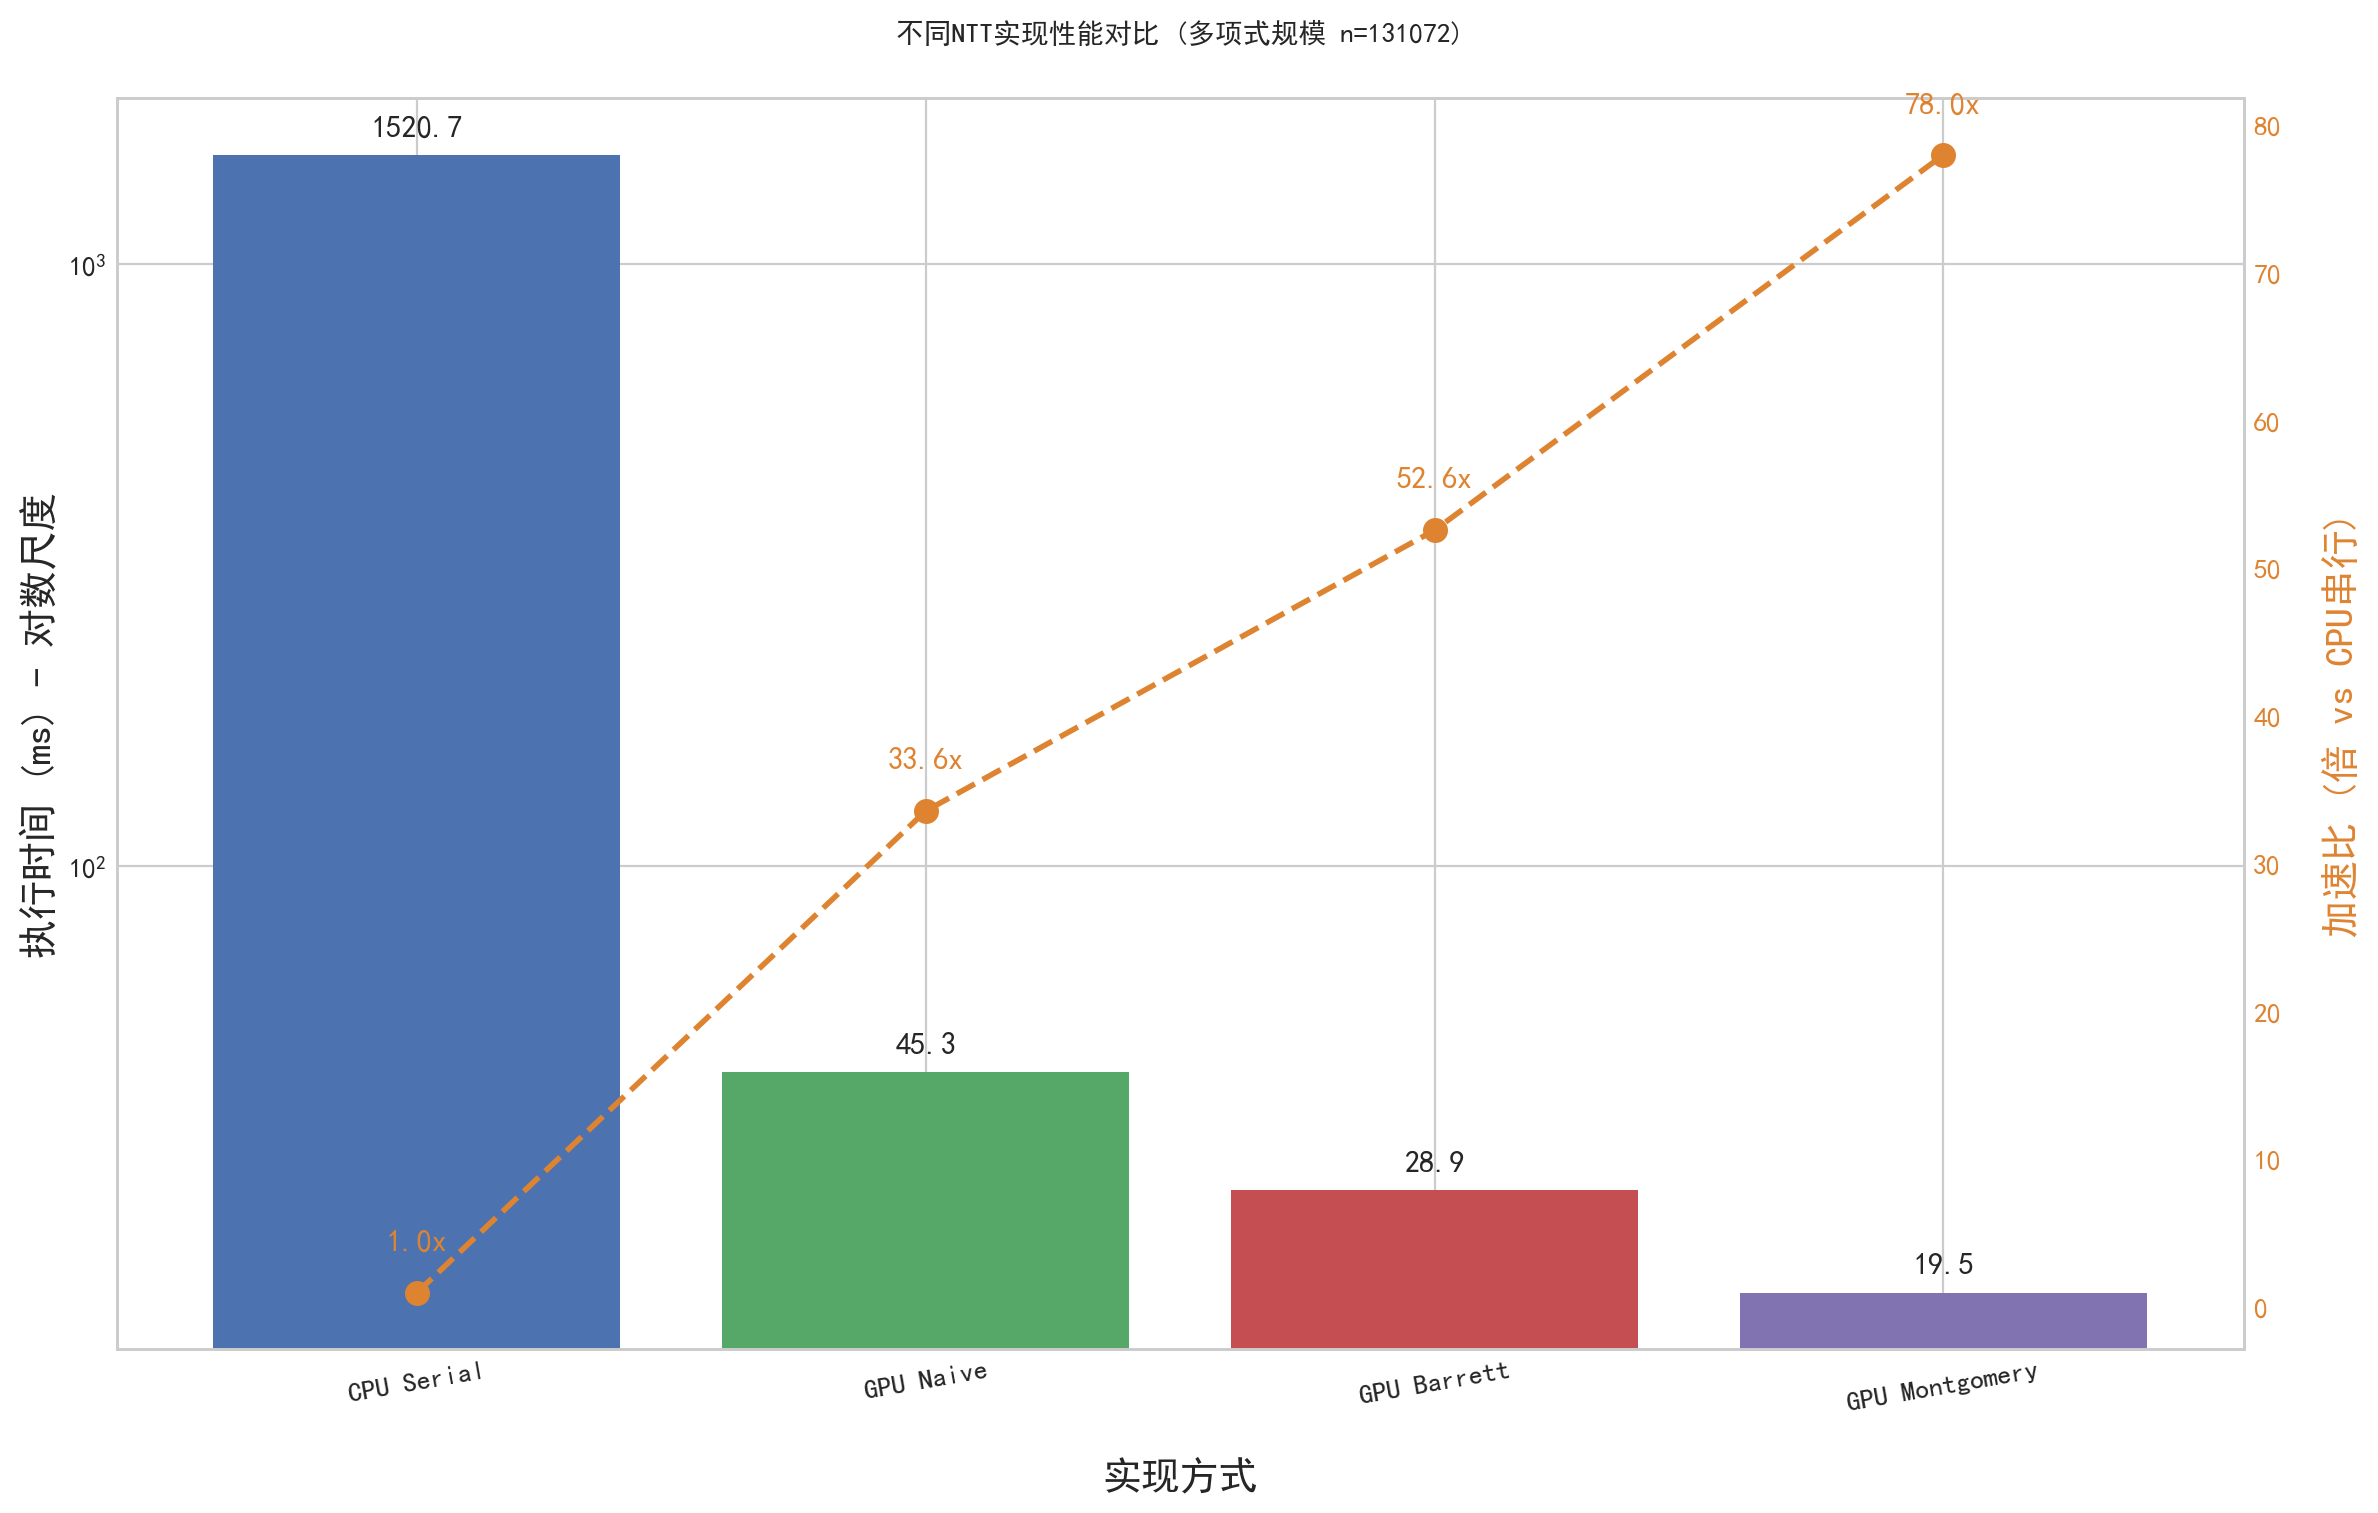
\includegraphics[width=0.8\textwidth]{fig/performance.png}
    \caption{GPU上不同模乘优化策略的性能对比}
    \label{fig:gpu_perf}
\end{figure}

\subsection{结果分析}
\begin{enumerate}
    \item \textbf{GPU vs CPU}: 从表中可以看出,最基础的GPU Naive版本相比于CPU串行版本获得了约 \textbf{33.6倍} 的加速比。这充分证明了GPU的大规模并行架构非常适合像NTT这样具有高度数据并行性的算法。

    \item \textbf{模乘优化的效果}:
    \begin{itemize}
        \item \textbf{Barrett vs Naive}: 使用Barrett约减的GPU版本比Naive版本快了约 \textbf{1.57倍} (45.3 / 28.9)。这表明通过将昂贵的硬件除法替换为更快的乘法和位运算,可以有效地提升内核的计算效率。
        \item \textbf{Montgomery vs Barrett}: 使用Montgomery约减的版本又比Barrett版本快了约 \textbf{1.48倍} (28.9 / 19.5)。尽管Montgomery需要额外的域转换开销,但在NTT这种需要海量模乘运算的场景下,其在域内极高的乘法效率带来了最佳的性能表现。
    \end{itemize}

    \item \textbf{综合性能}: 最终,经过完全优化的GPU Montgomery版本实现了相对于CPU串行版本高达 \textbf{78倍} 的惊人加速,展示了算法优化与硬件架构结合的巨大潜力。
\end{enumerate}

\section{结论}
本次实验成功地在CUDA平台上实现了多项式乘法的NTT算法,并通过一系列优化手段显著提升了计算性能。

主要成果包括:
\begin{itemize}
    \item 通过将NTT的蝶形运算并行化到GPU数千个线程上,获得了数十倍的基础性能提升。
    \item 设计并实现了一种高效的旋转因子管理策略,将主机与设备间的通信开销降至最低。
    \item 通过模板元编程,优雅地实现了三种不同模乘算法的对比测试。
    \item 实验数据证明,Barrett和Montgomery等高级模乘约减技术能有效避免硬件除法的瓶颈,带来显著的性能增益,其中Montgomery方法在NTT场景下表现最佳。
\end{itemize}

总的来说,本次实验不仅加深了对NTT算法和GPU并行编程的理解,也实际展示了如何通过软硬件结合的优化思想来解决计算密集型问题。

\end{document}